\documentclass[compress]{beamer}
%\usetheme{Warsaw}
\usepackage{graphics}
\usepackage{beamerthemesplit}
\usetheme[hoptionsi]{Madrid}
\usepackage{multicol}
 \title[Masters Dissertation]{Masters Dissertation}
 \subtitle {Adaptive And Interactive Smart Cafeteria Mobile Application}
 \logo{%
    
\includegraphics[width=1cm,height=1cm,keepaspectratio]{Logo/logo}~%
}
%\author[Supta R. Philip] % (optional, use only with lots of authors)
%{\textbf{Supta Richard Philip}~\inst{1}}
\author[Supta R. Philip]{\textbf{Supta Richard Philip}~\inst{1}\\{\small{Supervisor: Professor Antonella De Angeli}}}
% - Give the names in the same order as the appear in the paper.
% - Use the \inst{?} command only if the authors have different
%   affiliation.
\institute[University of Trento] % (optional, but mostly needed)
{
  \inst{1}%
  M.Sc. in Computer Science\\
  Department of Information Engineering
and Computer Science\\
  University of Trento, Italy.
  \\[\medskipamount]
     % 
\includegraphics[width=\textwidth,height=.5\textheight]{Logo/logo}%
      
\includegraphics[width=2.5cm,height=2.5cm]{Logo/logo}%
  %\\\scalebox{2}{\insertlogo}
  
  }
  
  
 \date [\today]{\today
%  \\ \ \\
%  \tiny{ Copywrite Declaration : Metarials are taken from Dr. Ashfaqur Rahman, Research Scientist,Intelligent Sensing and Systems Lab (ISSL),CSIRO, Australia \& \\
% Xiaohua Jia, Chair Professor,Dept of Computer Science,City University of Hong Kong.}
%  
 }
\AtBeginSection[]{
%   \setbeamercolor{section in toc shaded}{use=structure,fg=structure.fg}
%   \setbeamercolor{section in toc}{fg=mycolor}
%   \setbeamercolor{subsection in toc shaded}{fg=black}
%   \setbeamercolor{subsection in toc}{fg=mycolor}
  \frame<beamer>{\begin{multicols}{2}
  \frametitle{Outline}
  \setcounter{tocdepth}{2}  
  \tableofcontents[currentsection,subsections]
\end{multicols} 
 }
}


\begin{document}

{
 	 \begingroup
	\addtocounter{framenumber}{-1}
 	 %gets rid of bottom navigation bars
	\setbeamertemplate{footline}{}
	\setbeamertemplate{logo}{}
	%gets rid of navigation symbols
	\setbeamertemplate{navigation symbols}{}
 	\frame{
 	\addtocounter{framenumber}{0}
 	\titlepage
 	}
 	\endgroup
}

 \section*{Outline}
 \phantomsection
%\addcontentsline{toc}{sec}{Outline}
 \frame<beamer>{\begin{multicols}{2}
  \frametitle{Outline of Thesis}
  \setcounter{tocdepth}{2}  
  \tableofcontents
\end{multicols} 
 }

 
\section[]{Set of scenarios}
\begin{frame}\frametitle{Some title2}
The people who need the publications
 \begin{itemize}
 \item<1->  Hungry student
 \item<2-> Busy Professor
 \end{itemize}

\includegraphics[height=6cm,width=6cm]{abstract1.png} 
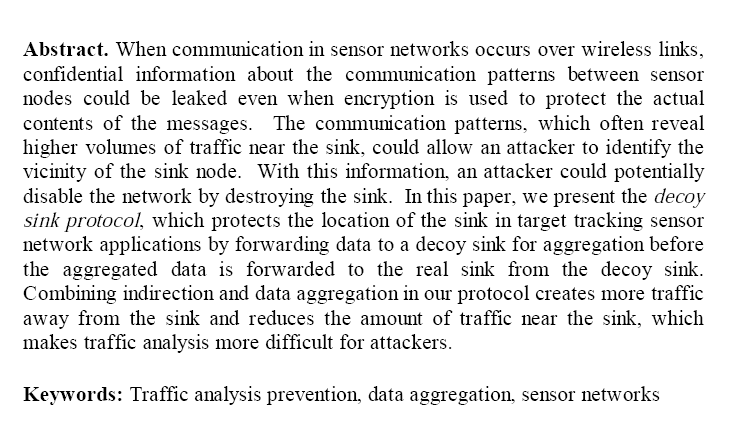
\includegraphics[height=6cm,width=5cm]{abstract.png} 
\end{frame}
\begin{frame}\frametitle{Some title2}Test\end{frame}

\section[Tools]{Automation}
\subsection{Overview}
\begin{frame}Test\end{frame}
\subsection{Littler}
\begin{frame}Test\end{frame}
\subsection{Rscript}
\begin{frame}Test\end{frame}

\section[Measure]{Measuring and Profiling}
\subsection{Overview}
\begin{frame}Test\end{frame}
\subsection{RProf}
\begin{frame}Test\end{frame}
\subsection{RProfmem}
\begin{frame}Test\end{frame}
\subsection[Profiling]{Profiling Compiled Code}
\begin{frame}Test\end{frame}
\subsection{Sumary}
\begin{frame}Test\end{frame}

\section[Faster]{Speeding up}
\subsection[Vec]{Vectorisation}
\begin{frame}Test\end{frame}
\subsection[Ra]{Just-in-time compilation}
\begin{frame}Test\end{frame}
\subsection{BLAS}
\begin{frame}Test\end{frame}
\subsection{GPUs}
\begin{frame}Test\end{frame}
\subsection{Summary}
\begin{frame}Test\end{frame}

\end{document}